
\chapter{Introducción al modelo Estándar}

\section{Introducción}
La física de partículas estudia los constituyentes universales del universo, esto es, las \textit{partículas elementales}, así como las interacciones entre estas. En la actualidad el modelo estándar es la teoría que mejor describe el comportamiento de estas partículas. Las partículas elementales descritas en el modelo se recogen en la siguiente imagen:

\begin{figure}[h!] \centering
	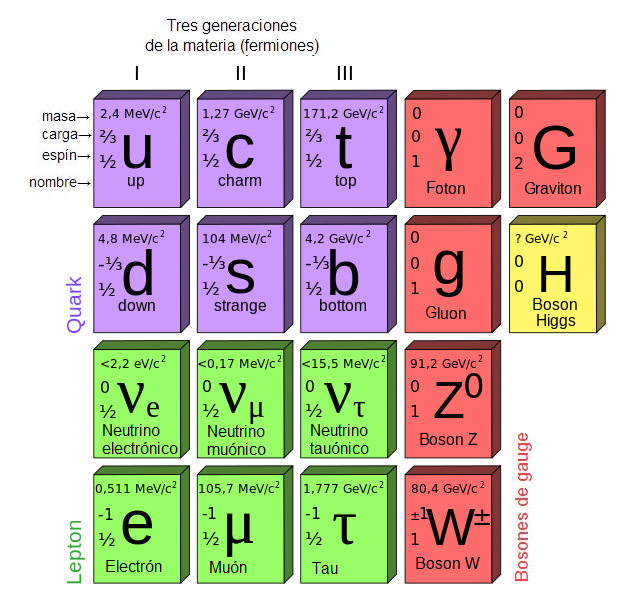
\includegraphics[width=0.65\textwidth]{Cuerpo/Ch_00/1_01_Modelo_Estandar.png}
	\caption{Partículas fundamentales según el modelo estándar}
\end{figure}


La \textit{dinámica} (que no la interacción) de los 12 fermiones fundamentales (leptones y quarks) está descrita por la ecuación de Dirac dentro del marco de la mecánica cuántica relativista. Esta ecuación nos dice que cada partícula tiene 2 estados posibles (uno con espín up +1/2 y otro con espín down -1/2).

Las fuerzas fundamentales nos dicen como interaccionan los diferentes fermiones entre sí, obteniendo entonces la siguiente tabla:

\begin{table}[h!] \centering
	\begin{tabular}{c|c c c}
		                  & Fuerte & Electromagnética & Débil \\ \hline
		Quarks            & Si     & Si               & Si    \\
		Leptones Cargados & No     & Si               & Si    \\
		Neutrinos         & No     & No               & Si    \\
	\end{tabular}
\end{table}

En el modelo estandar y la física de partículas moderna cada fuerza está descrito por un campo cuántico, todos ellos teorías gauge basados en un diferente grupo de de Lie, en particular nos gustan los grupos compactos y semi-simples, para obtener la teoría Young-Milles. En función de las características de cada fuerza, basaremos una u otra en la rotación de un grupo, que nos dará difernetes propiedades. En particular:

\begin{itemize}
	\item La descripción de la fuerza electromagnética se hace a través de la \textbf{elecrodinámica cuántica} (QED) teoría gauge basada en el grupo abeliano U(1). La \textit{carga conservada} asociada será la carga eléctrica.
	\item La descripción de la fuerza débil se hace a través de un grupo SU(2), pero su falta de precisión a la hora de describir ciertos fenómenos hace que la teoría que mejor la describa sea la SU(2) $\otimes$ U(1), es decir, la \textbf{teoría electrodébil} que engloba a la QED. La \textit{carga conservada} asociada será la el isospín débil.
	\item La descripción de la fuerza fuerte se hace a través de la \textbf{cromodinámica cuántica} y el grupo SU(3). La \textit{carga conservada} asociada será el color.
\end{itemize}
La descricpción de cada uno de estos se hace a través de bosones gauge con espin 1. El número de bosones gauge depende intrínsecamente del número de generadores del grupo de simetría. Por ejemplo, en el grupo U(1) solo tenemos un generador, por lo que solo habrá un bosón: el fotón $\gamma$. El grupo SU(3) tiene 8 generadores, por lo que habrá 8 bosones: los gluones. El grupo SU(2) tiene 3 generadores, por lo que habrá 3 bosones: W$^+$, W$^-$ y Z$^0$.

Luego para completar el modelo estándar tendremos que incluir el mecanismo que le da masa a los bosones que es el famoso mecanismo de Higgs, descubierto gracias a los experimentos ATLAS y CMS en el CERN LHC en 2012. Para este mecanismo de dar masa harían falta bosones escalares de espin 0: el bosson de Higgs con $m_H=125$ GeV/c$^2$. Este boson rompería espontánemanete la simetría gauge de las diferentes teorías.

\section{Los vértices del modelo estándar y constante de acopolo}

El acoplo de los de los bosones gauge a los fermiones está descrito por los lagrangianos de interaccion. En general se suele dar que un vértice contenga la interacción de un boson gauge y 2 particulas entrantes y/o salientes, asociadas a una \textbf{consatnte de acoplo adimensional} $g$. En el caso de QED tenemos que $g=|e|$ siendo $e$ adimensional a través de las unidades naturales ($\hbar = c = \varepsilon_0 =0$). En el

Además de la constante de acopolo $g$ tendremos el poder relativo $\alpha$ que nos da una medida de la fuerza de cada interaccion y las relaciones entre las fuerzas. En el caso de la fuerza electromangética esta esta relacionada con la constante de estructura fina $\alpha= e^2 / 4 \pi \approx 1/137$ pero no tiene porque tener la misma forma en cada una de las interacciones.

\begin{equation}
	\alpha_{QED} = \frac{1}{137} \qquad \alpha_{QCD} = 1 \qquad \alpha_{\text{weak}} = \frac{1}{30}
\end{equation}
\begin{minipage}{0.22\linewidth}
	\begin{tikzpicture}
		\begin{feynman}
			\vertex (f1) at (-1,1) {\(q\)};
			\vertex (f2) at (-1,-1) {\(\bar{q}\)};
			\vertex (ph) at (1,0) {\(g\)};
			\vertex [dot] (v) at (0,0) {};

			\diagram* {
				(f1) -- [fermion] (v) -- [anti fermion] (f2),
				(v) -- [gluon] (ph),
			};
		\end{feynman}
	\end{tikzpicture}
	\centering
\end{minipage}
\hfill
\begin{minipage}{0.22\linewidth}
	\begin{tikzpicture}
		\begin{feynman}
			\vertex (f1) at (-1,1) {\(f\)};
			\vertex (f2) at (-1,-1) {\(\bar{f}\)};
			\vertex (ph) at (1,0) {\(\gamma\)};
			\vertex [dot] (v) at (0,0) {};

			\diagram* {
				(f1) -- [fermion] (v) -- [anti fermion] (f2),
				(v) -- [photon] (ph),
			};
		\end{feynman}
	\end{tikzpicture}
	\centering
\end{minipage}
\hfill
\begin{minipage}{0.22\linewidth}
	\begin{tikzpicture}
		\begin{feynman}
			\vertex (f1) at (-1,1) {\(f^-\)};
			\vertex (f2) at (-1,-1) {\(\nu_f\)};
			\vertex (ph) at (1,0) {\(W^-\)};
			\vertex [dot] (v) at (0,0) {};

			\diagram* {
				(f1) -- [fermion] (v) -- [fermion] (f2),
				(v) -- [boson] (ph),
			};
		\end{feynman}
	\end{tikzpicture}
	\centering
\end{minipage}
\hfill
\begin{minipage}{0.22\linewidth}
	\begin{tikzpicture}
		\begin{feynman}
			\vertex (f1) at (-1,1) {\(f^-\)};
			\vertex (f2) at (-1,-1) {\(f^+\)};
			\vertex (ph) at (1,0) {\(Z\)};
			\vertex [dot] (v) at (0,0) {};

			\diagram* {
				(f1) -- [fermion] (v) -- [anti fermion] (f2),
				(v) -- [boson] (ph),
			};
		\end{feynman}
	\end{tikzpicture}
	\centering
\end{minipage}

\section{Diagramas de Feynman}

La represetnación de las interacciones entre partículas/estados en QFT se hace a través de los diagramas de Feynman, que incluyen todos los órdenes temporales posibles  

Desde la TCC es posible derivar las reglas de Feynman que nos permiten obtener las amplitudes de probabilidad a partir del esquema, con vértices y partículas virtuales. Una vez el diagrama es dibujado, es ``trivial'' calcular la amplitud  de probabilidad (también llamado \textit{elemento de matriz de transición}) siempre y cuando se conozcan estas reglas, evitando calcular cada proceso desde los prinicipios de la teoría cuántica de campos. 

Sin embargo para cada proceso de interaccion de varias partículas hay infinitos diagramas. Para la mayor parte de las interaccioens los diagramas que generan más amplitud son realmente los de bajo orden, que son los más sencillos de calcular. 



\subsection{Mandelstam variables}

Las variavles de mandelstam son 3 cantidades escalares que son invariantes en cualquier scattering 1+2$\to$3+4, sean leptones, neutrinos... Cada uno está asociado en general a uno de los 3 tipos de diagramas de Feynman que se pueden dibujar, y vienen dados por: 

\begin{itemize}
	\item La variable $s$ asociada a un proceso de aniquilación. Se le llama canal $s$ (\textit{space channel}): 
	\begin{equation}
		s = (p_1^2 + p_2^2)
	\end{equation}
	\item La variable $t$ asociada a un proceso de  scattering elástico. Se le llama canal $t$ (\textit{time channel}): 
	\begin{equation}
		t = (p_1^2 - p_3^2)
	\end{equation}
	\item La variable $u$ asociada a un proceso de scattering elástico. Se le llama canal $u$:
	\begin{equation}
		u = (p_1^2 - p_4^2)
	\end{equation}
	Este proceso es relevante cuando las partículas salientes son indistinguibles. 
\end{itemize}
El valor $\sqrt{s}$ es la energía total en el sistema centro de masas disponible. 

% Canal s
\begin{minipage}{0.32\linewidth}
\centering
\begin{tikzpicture}
  \begin{feynman}
    \vertex (i1) at (-1,1) {\(f_1\)};
    \vertex (i2) at (-1,-1) {\(\bar{f}_2\)};
    \vertex (v1) at (0,0);
    \vertex (v2) at (2,0);
    \vertex (f1) at (3,1) {\(f_3\)};
    \vertex (f2) at (3,-1) {\(\bar{f}_4\)};

    \diagram* {
      (i1) -- [fermion] (v1) -- [fermion] (i2),
      (v1) -- [boson, edge label=\(s\)] (v2),
      (v2) -- [fermion] (f1),
      (v2) -- [anti fermion] (f2),
    };
  \end{feynman}
\end{tikzpicture}
\end{minipage}
%
\hfill
% Canal t
\begin{minipage}{0.32\linewidth}
\centering
\begin{tikzpicture}
  \begin{feynman}
    \vertex (i1) at (-1,2) {\(f_1\)};
    \vertex (f1) at (1,2) {\(f_3\)};
    \vertex (i2) at (-1,-2) {\(\bar{f}_2\)};
    \vertex (f2) at (1,-2) {\(\bar{f}_4\)};
    \vertex (v1) at (0,1);
    \vertex (v2) at (0,-1);

    \diagram* {
      (i1) -- [fermion] (v1) -- [fermion] (f1),
      (i2) -- [anti fermion] (v2) -- [anti fermion] (f2),
      (v1) -- [boson, edge label=\(t\)] (v2),
    };
  \end{feynman}
\end{tikzpicture}
\end{minipage}
%
\hfill
% Canal u
\begin{minipage}{0.32\linewidth}
\centering
\begin{tikzpicture}
  \begin{feynman}
    \vertex (i1) at (-1,2) {\(f_1\)};
    \vertex (f1) at (1,2) {\(f_3\)};
    \vertex (i2) at (-1,-2) {\(\bar{f}_2\)};
    \vertex (f2) at (1,-2) {\(\bar{f}_4\)};
    \vertex (v1) at (0,1);
    \vertex (v2) at (0,-1);


    \diagram* {
      (i1) -- [fermion] (v1) -- [fermion] (f2),
      (i2) -- [anti fermion] (v2) -- [anti fermion] (f1),
      (v1) -- [boson, edge label=\(u\)] (v2),
    };
  \end{feynman}
\end{tikzpicture}
\end{minipage}